\documentclass[../main.tex]{subfiles}

\begin{document}

If $f$ and $g$ are functions, then for every $x$ that belongs to the domains
of both $f$ and $g$ we define functions

$(f+g)(x)=f(x)+g(x)$

$(f-g)(x)=f(x)-g(x)$

$(fg)(x)=f(x)g(x)$

$(f/g)(x)=f(x)/g(x)$ where $g(x)\neq 0.$

\begin{example}
Let $f(x)=\frac{1}{x+2}$ and $g(x)=\frac{x}{x-1}$. Find $(f+g)(x),(f-g)(x),$
$(fg)(x)=f(x)g(x)$ and $(f/g)(x)$ where $g(x)\neq 0.$
\end{example}

\subsection*{Composition of Functions}
If $f$ and $g$ are two functions, then
\[
  f\circ g(x)=f(g(x)).
\]
The domain of $f\circ g$ consists of those numbers $x$
in the domain of $g$ for which $g(x)$ is in the domain of $f$.


\begin{example}
  \begin{figure}[H]
    \centering
    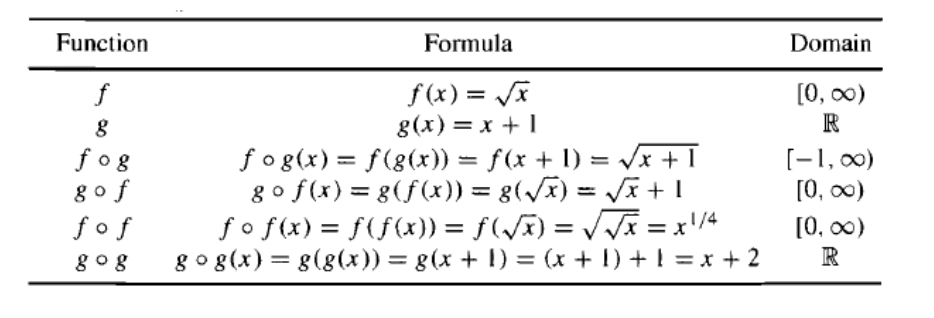
\includegraphics[width=0.95\textwidth]{P5-compfunc.png}
  \end{figure}
\end{example}
\subsection*{Piecewise Defined Functions}
Functions which are defined by different formulas on different intervals are sometimes called \textbf{piecewise defined functions.}

\begin{example}
  \[
  g(x) =
  \begin{cases}
      2x & \text{for } x<0 \\
      x^2 & \text{for }x\geq0
  \end{cases}
  \]
\end{example}


\subsection*{Inverse Functions}
Remember that a function is \textbf{one-to-one} if for every value in the range, there is exactly one value in the domain.

A function is one-to-one if every horizontal line crosses its graph at most once, which is commonly known as the \textbf{horizontal line test}.
\end{document}